\newpage
\section{Analisi dei Risultati}
\label{section:analisirisultati}

Prima di iniziare ad elencare i test effettuati e mostrare i risultati ottenuti, è
necessario sottolineare una questione relativamente importante.
Dopo aver visto come si comporta l'applicativo con grafi molto grandi (> 500 nodi) è stato ottenuto opportuno
abbassare il numero dei nodi affinchè l'esecuzione non portasse via troppo tempo e risorse.
Tutte le analisi sono state effettuate con reti composte da 500 nodi.
Un secondo punto da chiarire è che avendo due applicativi, 
il primo in Java per creare grafi (Capitolo~\ref{section:graph_topologies_dm}) e il secondo in NetLogo per utilizzarli nelle simulazioni,
è stato ritenuto opportuno non cambiare mai il grafo durante i test.


\subsection{Primo test}
\label{section:first_test}

In questa prima analisi verranno confrontati i due tipi di grafo descritti nel capitolo \ref{section:graph_topologies}.

Per questo test abbiamo bisogno di:
\begin{itemize}
\item un gruppo di utenti che forma il 100\% dei nodi;
\item un grafo di 500 nodi creato grazie all'algoritmo Preferential Attachment (Capitolo \ref{section:graph_topologies_pa});
\item un grafo di 500 nodi creato grazie all'algoritmo di Dorogovtsev e Mendes (Capitolo \ref{section:graph_topologies_dm});
\item un ciclo che vari la ``forza'' della notizia portandola da 0 a 1 con passi di 0.05.
\end{itemize}



\begin{figure}[!ht]
  \begin{subfigure}[l]{0.5\textwidth}
    \begin{center}
      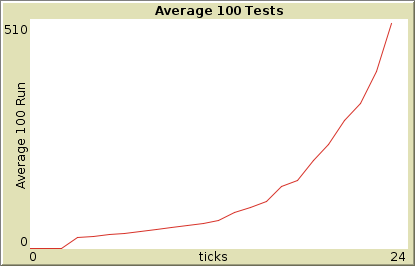
\includegraphics[width=1\textwidth]{img/interface-test-1-preferential-attachment-chart.png}
    \end{center}
    \caption{Con Preferential Attachment}
    \label{img:result_test_1_pa}
  \end{subfigure}
  \begin{subfigure}[r]{0.5\textwidth}
    \begin{center}
      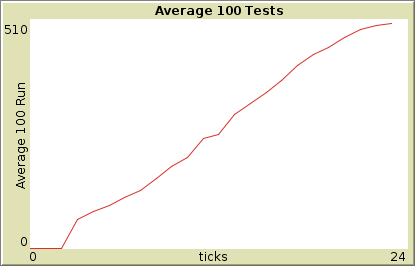
\includegraphics[width=1\textwidth]{img/interface-test-1-dorogovtsev-mendes-chart.png}
    \end{center}
    \caption{Con Dorogovtsev e Mendes}
    \label{img:result_test_1_dm}
  \end{subfigure}
 \caption{Risultati del primo test}
 \label{img:graph_models}
\end{figure}


Con il grafo descritto da Barabási e Albert si ottiene il risultato che viene mostrato nel grafico di figura \ref{img:result_test_1_pa}.
Come si nota ha una crescita molto lenta e solo dopo che la probabilità di condivisione ha superato il valore di 0.5 si ha una salita.
La topologia descritta da Dorogovtsev e Mendes invece si comporta molto meglio e viene mostrata nel grafico in figura \ref{img:result_test_1_dm}.
Ha una crescita quasi lineare e alla fine, quando la forza è attorno l'85\% crea una ``pancia'' verso l'alto che sta a dimostrare l'altissima 
condivisione.

Il primo grafo è molto svantaggiato per via della sua struttura. Come abbiamo detto in fase di progettazione (Capitolo \ref{section:progettazione}) 
questo grafo non presenta cricche al suo interno.
Questa proprietà lo penalizza nelle simulazioni che sono basate sul numero di visualizzazioni e perciò sulla probabilità di condivisione.
Nel modello descritto da Dorogovtsev e Mendes invece sono presenti cricche al suo interno e possiede quasi il doppio dei link del Preferential Attachment.

Per i motivi appena esposti si è optato di affrontare i prossimi test con la seconda topologia.

Inoltre, anche se è solo un punto di vista dell'autore, si può notare in questo modello di grafo una 
maggior somiglianza con la topologia più comune di un Social Network.


\subsection{Secondo test}
\label{section:second_test}




\subsection{Terzo test}
\label{section:third_test}

In quest'ultima analisi, invece, verrà mostrata un'interazione tra 2 diversi gruppi di utenti (Nodi).
Il primo gruppo è formato da persone con una maggior probabilità di condividere la notizia 
mentre nel secondo, al contrario, da persone con una minor probabilità.
Questo studio punta ad analizzare quante visualizzazioni vengono fatte per una singola informazione condivisa.
Verrà anche condotto uno studio in cui il totale degli utenti si divide in due gruppi costituiti da, ad esempio, 
pochi utenti con alte probabilità di condividere l'informazione e, viceversa, 
molti utenti con basse probabilità di condivisione.

La possibilità di condivisione è data nuovamente dal confronto tra la ``forza della notizia'' e la ``forza di astensione''. 
In questo caso, però, l'astensione viene calcolata tramite una funzione di distribuzione di probabilità non lineare,
quella scelta è la funzione Weibull già descritta al capitolo~\ref{section:great_sharers_vs_little_sharers}.

Per ottenere una curva di distribuzione più o meno inclinata, in seguito ai tentativi attuati, 
è stato ritenuto opportuno mantenere il valore di $\beta$ costante a 1.0 e variare, invece, quello di $\alpha$.

Il valore di $\alpha$ per il secondo gruppo invece è stato fissato a 0.75 perchè 
la distribuzione di figura~\ref{img:weibull_alpha_0_75} mostra un dislivello non troppo 
alto che consente, comunque, un buon grado di condivisione della notizia.

Riassumendo il test viene composto da i parametri dinamici citati nel 
capitolo~\ref{section:great_sharers_vs_little_sharers} e dai seguenti parametri statici:
\begin{itemize}
\item La dimensione della popolazione non cambia mai e resta sempre di 500 Nodi;
\item Il parametro $\alpha$ del gruppo con bassa probabilità di condivisione rimane $0.75$, 
ottenendo una densità di probabilità come in figura \ref{img:weibull_alpha_0_75};
\item La topologia del grafo è la stessa per ogni esecuzione del test;
\end{itemize}


\begin{figure}[!ht]
\centerline {
  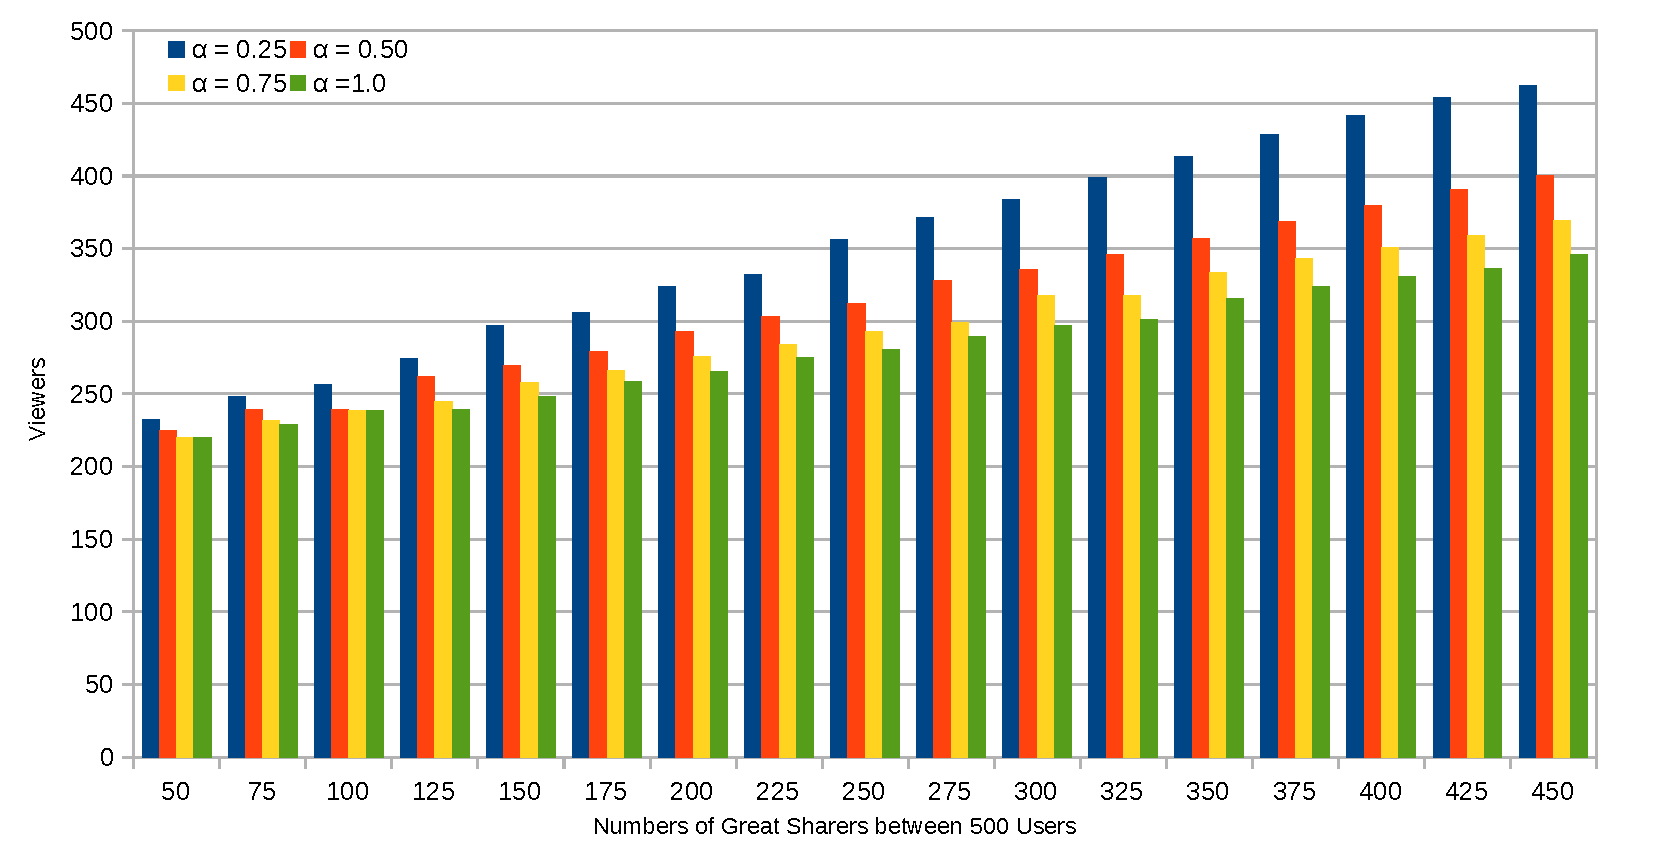
\includegraphics[width=1\textwidth]{charts/last-test-str_0.5.pdf}
}
\caption{Grafico del risultato dell'ultimo test con forza della notizia pari a $0.50$, 
500 nodi totali e $\alpha$ del gruppo con bassa probabilità di condivisione = $0.75$}
\label{img:last_test_str_0_5}
\end{figure}

La figura \ref{img:last_test_str_0_5} mostra il risultato atteso, 
ovvero la crescita del numero di visualizzazioni sia al variare di $\alpha$ che all'aumentare 
dei nodi con alta probabilità di condivisione.

Si vuole inoltre porre l'attenzione su come con un valore di $\alpha$ 
molto basso ($0.2$) ed un numero di nodi con alta probabilità di condivisione pari a 150 corrisponda 
a ~ 300 visualizzazioni totali, quasi le stesse ottenute da un valore di $\alpha$ = 1.0 e 325 nodi con 
alta probabilità di condivisione.















